\documentclass[b5paper]{book}
\usepackage[
    b5paper,
		margin=2cm,
	]{geometry}
\setlength\parindent{0em}
\setlength{\parskip}{1em}

\usepackage{booktabs}
\usepackage{blindtext}

%-----------%
% XREF DICT %
%-----------%

\usepackage{pgfkeys}
\pgfkeyssetvalue{/xref dict/fig}{Figure}
\pgfkeyssetvalue{/xref dict/eq}{Equation}
\pgfkeyssetvalue{/xref dict/eqs}{Equations}
\pgfkeyssetvalue{/xref dict/tab}{Table}
\pgfkeyssetvalue{/xref dict/def}{Definition}
\pgfkeyssetvalue{/xref dict/note}{Note}
\pgfkeyssetvalue{/xref dict/challange}{Challange}
\pgfkeyssetvalue{/xref dict/example}{Example}

%----------%
% GRAPHICS %
%----------%

\usepackage{caption}
\usepackage{subcaption}

\usepackage{tikz}
\usepackage{tikzpagenodes}
\usetikzlibrary{positioning, calc, decorations.pathreplacing, decorations.text}

\tikzset{
	arrow/.style={thick, ->, >=stealth},
	vector/.style={very thick, ->, >=stealth},
}

\usepackage{pgfplots}
\usepgfplotslibrary{fillbetween, colormaps, colorbrewer}
\pgfplotsset{
		compat=1.16,
		every axis/.append style={
			font=\small,
		},
		graph2d/.style={
		axis x line=middle,
		axis y line=middle,
		every axis x label/.style={
			at={(ticklabel* cs:1.01)},
			anchor=west,
		},
		every axis y label/.style={
			at={(ticklabel* cs:1.01)},
			anchor=south,
		},
		axis line style={stealth-stealth, thick},
		label style={font=\large},
		xlabel=$x$,
		ylabel=$y$,
		tick label style={font=\small},
		samples=200,
		grid=both,
		grid style={line width=.1pt, draw=gray!20},
		major grid style={line width=.2pt,draw=gray!50},
		minor tick num=4,
	},
	function/.style={line width=1.5pt},
}

%-------%
% FONTS %
%-------%

\usepackage{kpfonts}

%--------%
% COLORS %
%--------%

\usepackage{xcolor}
\usepackage{colortbl}
\definecolor{xblue}{HTML}{4268BD}
\definecolor{xred}{HTML}{BD4242}
\definecolor{xgreen}{HTML}{52B256}
\definecolor{xpurple}{HTML}{7F52B2}
\definecolor{xorange}{HTML}{FF9F31}
\definecolor{xdotted}{HTML}{999999}

% Document-specific colors
\colorlet{normaltextcolor}{black}
\colorlet{figtextcolor}{xblue}

%------- %
% XHFILL %
%------- %

\usepackage{xhfill}

%---------------%
% CHAPTER TITLE %
%---------------%

% Used to set chapter title look.
% "explicit" is there so we can
% use the first parameter (#1).
\usepackage[explicit]{titlesec}
\newcommand{\chapternumsize}{\fontsize{70}{70}\selectfont}
\newcommand{\chaptertitlesize}{\fontsize{30}{30}\selectfont}

\titleformat{\chapter}{\sffamily\bfseries}{}{0pt}{
	\centering
	\begin{tikzpicture}[font=\sffamily\bfseries]
		\fill[black!10, rounded corners] (0,0) rectangle (5cm,5cm);
		\node (chapternum) at (2.5cm,4.5cm) {\fontsize{85}{85}\selectfont\thechapter};
		\node[below of=chapternum, yshift=-2cm] {
\includegraphics[scale=1.5]{figures/chapters/tapir_rainbow.pdf}};
		\node[align=center, below of=chapternum, yshift=-5cm] {\fontsize{30}{30}\selectfont\uppercase{#1}};
		\node[align=center, above of=chapternum, yshift=5mm] {\huge CHAPTER};
	\end{tikzpicture}
}

\titleformat{\section}{\sffamily\Large\bfseries}{\huge{\thesection}}{1em}{\uppercase{#1}}

\titleformat{\subsection}{\sffamily\large\bfseries}{}{0em}{\uppercase{#1}}

%------------%
% REFERENCES %
%------------%
\usepackage{chngcntr}
\counterwithin{table}{chapter}
\counterwithin{figure}{chapter}
\renewcommand{\eqref}[1]{
	Equation \ref{eq:#1}
}
\newcommand{\tabref}[1]{
	\textbf{\textcolor{xblue}{Table} \ref{tab:#1}}
}
\newcommand{\figref}[1]{
	\textbf{\textcolor{xblue}{Figure} \ref{fig:#1}}
}
\newcommand{\noteref}[1]{
	\textbf{\textcolor{xred}{Note} \ref{note:#1}}
}
\newcommand{\exampleref}[1]{
	\textbf{\textcolor{xblue}{Example} \ref{example:#1}}
}

%---------%
% HEADERS %
%---------%

\usepackage{fancyhdr}
\pagestyle{fancy}
\fancyhf{}% Clear header/footer
\renewcommand{\chaptermark}[1]{\markboth{\chaptername\ \thechapter:\ #1}{}}
\fancyhead[RO,LE]{\leftmark}% Chapter details in book
\fancyfoot[RO,LE]{\thepage}
\makeatother

%-------%
% BOXES %
%-------%

\usepackage{fontawesome}
\usepackage[most]{tcolorbox}
\tcbset{
	common/.style={
		lower separated=false,
		coltitle=white,
		colback=gray!5,
		boxrule=0.5pt,
		fonttitle=\bfseries,
		enhanced,
		breakable,
		top=8pt,
		before skip=8pt,
		attach boxed title to top left={
			yshift=-0.25cm,
		xshift=0.38cm},
		boxed title style={
			boxrule=0pt,
			colframe=white,
			arc=0pt,
		outer arc=0pt},
	separator sign={~~},},
	defstyle/.style={
		common,
		colframe=xpurple,
		colback=xpurple!5,
		colbacktitle=xpurple,
		overlay unbroken and last={
			\node[anchor=south east, outer sep=0pt] at (\linewidth-width, 0) {
	\textcolor{xpurple}{$\pi$}};}},
	exmplstyle/.style={
		common,
		colframe=xblue,
		colback=xblue!5,
		colbacktitle=xblue,
		overlay unbroken and last={
			\node[anchor=south east, outer sep=0pt, font=\large\bfseries] at (\linewidth-width, 1) {
	\textcolor{xblue}{\faArrowCircleDown}};}},
	notestyle/.style={
		common,
		colframe=xred,
		colback=xred!5,
		colbacktitle=xred,
		overlay unbroken and last={
			\node[anchor=south east, outer sep=0pt, font=\large\bfseries] at (\linewidth-width, 1) {
	\textcolor{xred}{!}};}},
	chllngstyle/.style={
		common,
		colframe=xgreen,
		colback=xgreen!5,
		colbacktitle=xgreen,
		overlay unbroken and last={
			\node[anchor=south east, outer sep=0pt, font=\large\bfseries] at (\linewidth-width, 0) {
	\textcolor{xgreen}{?}};}},
	thmstyle/.style={
		common,
		colframe=second,
		colback=second!5,
		colbacktitle=second,
		overlay unbroken and last={
			\node[anchor=south east, outer sep=0pt] at (\linewidth-width,0) {
	\textcolor{second}{$\heartsuit$}};}},
	theoremstyle/.style={
		common,
		colframe=xpurple,
		colback=xpurple!5,
		colbacktitle=xpurple,
		overlay unbroken and last={
			\node[anchor=south east, outer sep=0pt, font=\large\bfseries] at (\linewidth-width, 1) {
	\textcolor{xpurple}{$\multimapdotbothA$}};}},
}
\newtcbtheorem[auto counter, number within=chapter]{definition}{Definition}{defstyle}{def}
\newtcbtheorem[auto counter, number within=chapter]{example}{Example}{exmplstyle}{example}
\newtcbtheorem[auto counter, number within=chapter]{note}{Note}{notestyle}{note}
\newtcbtheorem[auto counter, number within=chapter]{challange}{Challange}{chllngstyle}{challange}
\newtcbtheorem[auto counter, number within=chapter]{theorem}{Theorem}{theoremstyle}{theorem}

%---------%
% FIGURES %
%---------%

\usepackage{float}
\usepackage{caption}
\usepackage[colorlinks=true, linkcolor=xblue]{hyperref}

% Caption label
\DeclareCaptionLabelSeparator{doublespace}{\ \ }
\captionsetup{labelfont={color=xblue,bf}, figurename=Figure, labelsep=doublespace}

% Refs format
\newcommand{\xref}[2][fig]{
	\color{figtextcolor}\textbf{\pgfkeysvalueof{/xref dict/#1}}~\ref{#1:#2} \color{normaltextcolor}
}

%-------------------%
% HIGHLIGHTED WORDS %
%-------------------%

\usepackage{imakeidx}
\usepackage{marginnote}
\makeindex
\renewcommand\emph[1]{\color{xpurple}{\textbf{#1}}\color{normaltextcolor}\index{#1}}%\marginnote[#1]{}

%-------%
% MATHS %
%-------%

\usepackage{amsmath, bm}
\numberwithin{equation}{chapter}
\usepackage{siunitx}
\newcommand{\Rs}[1]{\mathbb{R}^{#1}}
%\newcommand{\true}{\colorbox{xblue!25}{true}}
%\newcommand{\false}{\colorbox{xred!25}{false}}
\newcommand{\true}{\textcolor{xblue}{\textbf{true}}}
\newcommand{\false}{\textcolor{xred}{\textbf{false}}}
\newcommand{\AND}{\textbf{AND}}
\newcommand{\OR}{\textbf{OR}}
\newcommand{\opand}{\wedge}
\newcommand{\opor}{\vee}
\newcommand{\falseprop}[1]{
	\begingroup
	\color{xred}
	\underset{\false}{#1}
	\endgroup
}
\newcommand{\trueprop}[1]{
	\begingroup
	\color{xblue}
	\underset{\true}{#1}
	\endgroup
}
\newcommand{\defeq}{:=}
\newcommand{\eqdef}{=:}

%-------------%
% OTHER STUFF %
%-------------%
\usepackage[version=4]{mhchem}

%----------%
% DOCUMENT %
%----------%

\begin{document}

% Chapters
\setcounter{chapter}{-1}
\chapter{Introduction}
In this chapter we will introduce some key concepts that will be used in later chapters.

\begin{note}{In case you are already familiar with the topics}{}
	It is recommended for readers who are familiar with the topics to at least gloss over this chapter and make sure they know and understand all the concept presented here.
\end{note}

\section{Trigonometry}
Consider a \emph{right triangle} with sides $a,b,c$ and angles $\alpha, \beta, \gamma=\ang{90}$ (\figref{righttriangle}). We use the ratios between the three sides of the triangle to define three functions of $\alpha$:
\begin{definition}{The basic triginometric functions}{}

	\vspace{5mm}
	\begin{itemize}
		\item The \emph{sine} of the angle $\alpha$ is $\sin(\alpha)=\frac{a}{c}$.
		\item The \emph{cosine} of the angle $\alpha$ is $\cos(\alpha)=\frac{b}{c}$.
		\item The \emph{tangent} of the angle $\alpha$ is $\tan(\alpha)=\frac{b}{a}$.
		\end{itemize}
	\label{def:basic_trig}

\begin{figure}[H]
	\centering
	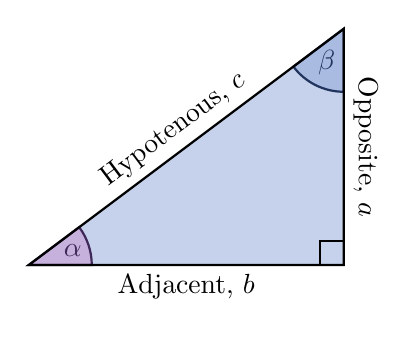
\begin{tikzpicture}
		\coordinate (A) at (0,0);
		\coordinate (B) at (4,3);
		\coordinate (C) at (4,0);

		\draw[fill=xblue!30] (A) -- node (c) [midway, above, rotate=36.87] {Hypotenous, $c$} (B) -- node (a) [midway, above, rotate=-90] {Opposite, $a$} (C) -- node (b) [midway, below] {Adjacent, $b$} cycle;
		\draw[thick] ($(C)+(0,0.3)$) rectangle ($(C)-(0.3,0)$);
		\draw[thick, xpurple!50!black, fill=xpurple!45] (A) -- ($(A)+(0.8,0)$) arc (0:36.87:0.8) node [midway, xshift=-2mm, yshift=-2pt] {$\alpha$} -- cycle;
		\draw[thick, xblue!50!black, fill=xblue!45] (B) -- ($(B)+(0,-0.8)$) arc (270:216.97:0.8) node [midway, above, xshift=4pt] {$\beta$} -- cycle;
		\draw[thick] (A) -- (B) -- (C) -- cycle;
	\end{tikzpicture}
	\caption{A right right triangle with sides $a,b,c$ and angles $\alpha,\beta,\gamma=\ang{90}$.}
	\label{fig:righttriangle}
\end{figure}
\end{definition}
\section{Sets}


% For tests
\chapter{This is a Test Title}
\section{The Foo and the Bar}
\subsection{The Foo; or: Why Does a Fish?}
\Blindtext
\begin{definition}{The Foo}{}
	A Foo is simply a thing, i.e.
	\begin{equation}
		e^{i\pi} = -e^{i\tau} = -1.
		\label{eq:a thing}
	\end{equation}
\end{definition}
\Blindtext[1]
\begin{example}{A Bla which is not a Foo}{}
	Is there even such a thing? Consider
	\begin{equation*}
		f(x) = \sin(x)+5x^{2}.
	\end{equation*}
\end{example}
\subsection{The Bar, the One and Only}
\Blindtext[3]
\begin{note}{Something to Consider}{}
	Bla bla bla, yada yada yada.
	~\\
	~\\
	More lines.
\end{note}
\Blindtext[2]

In the middle of this random Lorem Ipsum, there are some other words! This is refreshing, isn't it? Any way, this is used to test some \emph{highlighting} and \emph{indexing} of words. I hope it works. Well, it doesn't. I need to check how to make the marginnotes to go to the left side in odd pages.

\Blindtext[2]
\begin{challange}{Generalize this thing}{}
	In 2D, the distance between two points $\bm{A}=(A_{x},A_{y})$ and $\bm{B}=(B_{x},B_{y})$ is
	\begin{equation}
		|AB| = \sqrt{(A_{x}-B_{x})^{2} + (A_{y}-B_{y})^{2}}.
		\label{eq:dist2D}
	\end{equation}
	Generalize this to 3D and to $N$D, where $N\in\mathbb{N}$.
\end{challange}

\Blindtext[1]

As you probably learned in school, a \emph{triangle} is a shape with three sides. An example of a triangle can be seen in \xref{triangle}.

\begin{figure}[H]
	\centering
	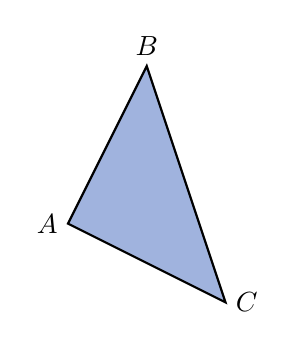
\begin{tikzpicture}
		\draw[thick, fill=xblue!50] (0,0) node [left] {$A$} -- (1,2) node [above] {$B$} -- (2,-1) node [right] {$C$} -- cycle;
	\end{tikzpicture}
	\caption{This is a triangle.}
	\label{fig:triangle}
\end{figure}

\stepcounter{chapter}
\printindex
\end{document}
